\section{Фактор-пространство}
Факторизирането е познато от други области като линейната алгебра и теория на групите, където разглеждаме множество елементи като един под действието на някакво изображение. По подобен начин ще разглеждаме и фактор-пространствата в топологията.

Има разнообразни начини да се въведе факторизирането. Нека се спрем на представянето чрез релация на еквивалентност.

\subsection{Силно непрекъснато изображение}
\begin{definition}
    Нека $X, Y$ са топологични пространства
    
    $p: X \to Y$. $p$ е силно непрекъснато изображение $\bydef$ p е сюрекция и $\forall U \in Y$ - отворено множество: $p^{-1}(U)$ е отворено множество в $X$
\end{definition}
\begin{definition}
    Нека $X$ е топологично пространство
    
    $C \subseteq X$ е наситено(спрямо сюрективно изображение $p: X\to Y$) $\bydef$ $\forall y \in X:\; p^{-1}(\{y\}) \cap C \neq \emptyset \rightarrow p^{-1}(\{y\}) \subseteq C$  
\end{definition}
\begin{notation}
    Когато е ясно от контекста ще пропускаме "спрямо сюрективно изображение \dots"
\end{notation}
Иначе казано, $C$ е наситено точно тогава когато има такова подмножество на $U \subseteq Y$, че $p^{-1}(U) = C$

Значи можем еквивалентно дДефинираме силно непрекъснато изображение чрез наситени множества
\begin{proposition}
    $p: X \to Y$ е силно непрекъсната $\iff$ $p$ е непрекъснато изображение и изобразява наситените отворени множества на $X$ в отворени множества на $Y$.
\end{proposition}

Лесно може да се съобрази, че:
\begin{proposition}
    Нека $X, Y$ са топологични пространства..

    $p: X \to Y$ е сюрективно непрекъснато отворено/затворено изображение $\Rightarrow$ $p$ е силно непрекъснато
\end{proposition}
\begin{remark}
    Това е достатъчно, но не е необходимо условие, т.е. има силно непрекъснати изображения, които не са нито отворени, нито затворени.
\end{remark}
\begin{proof}
    Нека разглеждаме $\pi_1: \R \to \R$. Нека $A$ е подпространство на $\R \times \R$, т.ч.:
    \begin{equation}
        A = \{\langle x, y \rangle \mid x \geq 0 \lor y=0\}
    \end{equation}
    Нека $q : A \to \R$ дефинирано като рестрикцията на $\pi_1$ върху $A$.

    Тогава твърдим, че $q$ не е нито отворено, нито затворено изображение.

    \begin{itemize}
        \item[(не е отворено)] Търсим такова отворено множество $X \subseteq A$, че $q(X)$ не е отворено в стандартната топология на $\R$.
        
        Нека $X = [0; 1) \times \{0\}$. Тогава:
        \begin{equation}
            q(X) = [0; 1)
        \end{equation}
        Но това не е отворено множество $\R$

        \item[(не е затворено)] Търсим такова затворено множество $X \subseteq A$, че $q(X)$ не е затворено в стандартната топология на $\R$.
        
        Нека $X = [0; 1) \times \{0\}$. Тогава:
        \begin{equation}
            q(X) = [0; 1)
        \end{equation}
        Но това не е затворено множество $\R$
    \end{itemize}
    Значи можем да използваме един и същи контрапример за двата случая понеже интервалът $[0; 1)$ не е нито отворен, нито затворен.

    Не можем да изразим като крайно/безкрайно обединение и сечение на отворени интервали - няма как да "затворим" отляво интервала.
    \begin{equation}
        [0; 1) = \{0\} \cup (0; 1)
    \end{equation}
    Защото $\{0\}$ не е отворено множество.

    Допълнението му също не е отворено множество:
    \begin{equation}
        \overline{[0; 1)} = (-\infty; 0) \cup [1; \infty) = \bigcup_{n \in \N} (-n;0) \cup \{1\} \cup \bigcup_{n\in\N} (1+n;\infty)
    \end{equation}
    Защото $\{1\}$ не е отворено множество
\end{proof}

\subsection{Фактор-топология дефинирана от изображение}
\begin{definition}
    Нека $X$ е топологично пространство, $A$ е произволно множество, $p: X \to A$ e сюрективно изображение

    Тогава единствената топология $\mathcal T$ над $A$, т.ч. $p$ е силно непрекъснато изображение, се нарича Фактор-топология породенa от $p$.

    \begin{equation}
        \mathcal T = \{U \subseteq A \mid p^{-1}(U) \in \mathcal T_X\}
    \end{equation}
\end{definition}
Лесно се проверява, че е топология - при съмнение \cite[стр.~138]{munkrestopology}

\begin{example}
    Нека $x \in \R$ е произволно и $A = \{a, b, c\}$ и $p: \R \to A$ дефинирано по следния начин:
    \begin{equation}
        p(y) = \begin{cases}
            a &, y > x\\
            b &, y < x\\
            c &, y = x
        \end{cases}
    \end{equation}

    Визуално топологията изглежда по следния начин:
    \begin{figure}[H]
        \centering
        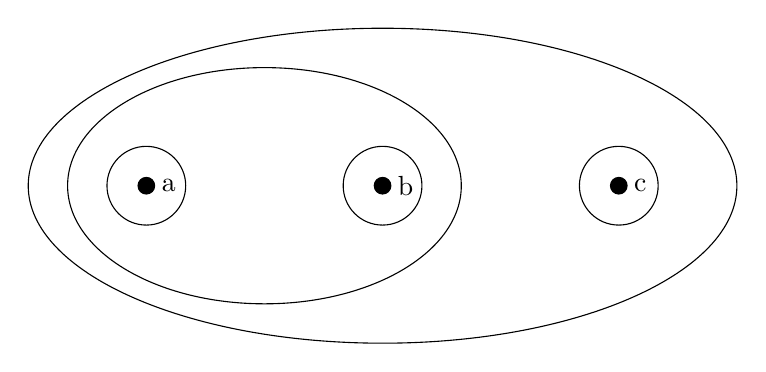
\begin{tikzpicture}
            \filldraw (-3, 0) circle (3pt) node [xshift = 2pt, anchor=west]{a};
            \filldraw (0, 0) circle (3pt) node [xshift = 2pt, anchor=west]{b};
            \filldraw (3, 0) circle (3pt) node [xshift = 2pt, anchor=west]{c};

            \draw (-3, 0) circle (0.5);
            \draw (0, 0) circle (0.5);
            \draw (3, 0) circle (0.5);
            \draw (-1.5, 0) ellipse (2.5 and 1.5);
            \draw (0, 0) ellipse (4.5 and 2);
        \end{tikzpicture}
        \caption{Визуално представяне на топологията породена от $p$}
    \end{figure}
\end{example}

\subsection{Фактор-пространство дефинирано от релация на еквивалентност}
\subsubsection{Припомняне от теория на множествата}
\begin{definition}
    Нека $X$ е множество, а $\sim$ релация над $X$.

    $\sim$ е релация на еквивалентност $\bydef$ $\sim$ е рефлексивна, симетрична и транзитивна.
\end{definition}
\begin{definition}
    Нека $X$ е множество, а $\sim$ релация на еквивалентност над $X$. Клас на еквивалентност породен от $x \in X$ наричаме множество от всички елементи еквивалентни на $x$:
    \begin{eqnarray}
        [x] \overset{def}{=} \{y \in X \mid x \sim y \}
    \end{eqnarray}
\end{definition}

\begin{definition}
    Нека $X$ е множество, а $\sim$ релация на еквивалентност над $X$. $X$ факторизирано по $\sim$ наричаме фамилия от множества съставена от всички класове на еквивалентност:
    \begin{eqnarray}
        X/_\sim = \left\{[x] \mid x \in X\right\}
    \end{eqnarray}
\end{definition}

\begin{fact}
    Лесно се проверява, че два класа или съвпадат, или са непресичащи се:
    \begin{eqnarray}
        [x] \cap [y] = \begin{cases}
            [x] = [y] &, x \sim y\\
            \emptyset &, x \not\sim y
        \end{cases}
    \end{eqnarray}
\end{fact}

\begin{corollary}
    $X/_\sim$ е разбиване на $X$
\end{corollary}
\begin{corollary}
    $X/_\sim$ поражда естествено сюрективно изображение $p: X \to X/_\sim,\; x \mapsto [x]$
\end{corollary}

\subsubsection{Фактор-пространство}
\begin{definition}
    Нека $X$ е множество, $\sim$ е релация на еквивалентност над $X$, с естествено влагане $p: X \to X/_\sim$. С топологията породена от $p$, $\langle X, X/_\sim\rangle$ се нарича фактор-пространство.
\end{definition}
